\section{Analisi dei Requisiti}
\labelsec{ReqAnalysis}
%===========================================================================
\subsection{Casi D'Uso}
\labelssec{UseCases}

\begin{figure}[ht]
\centering
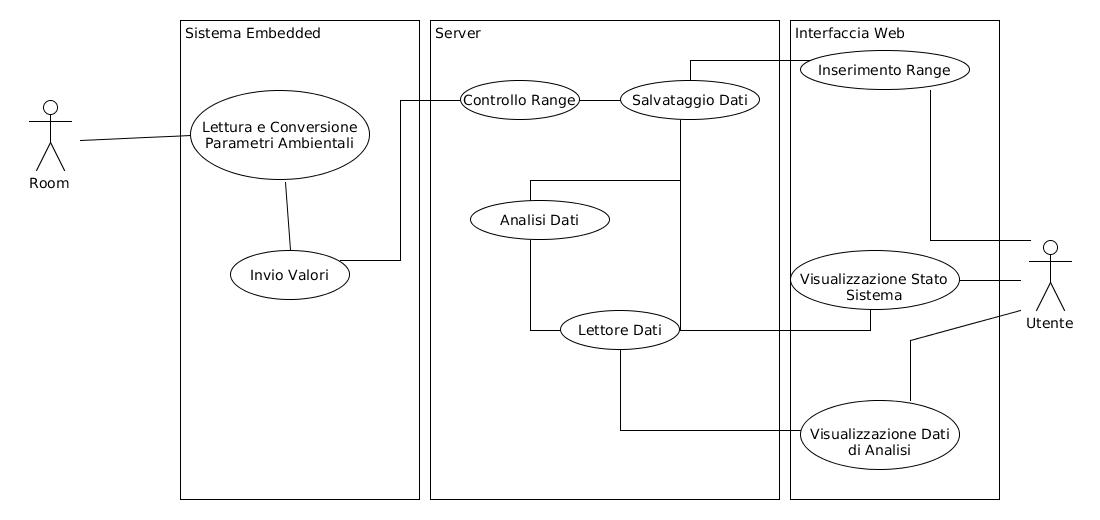
\includegraphics[width=\textwidth]{Figures/UseCases.jpg}
\caption{Casi d'Uso}
\end{figure}

Nell'immagine sopra si possono vedere quali sono le macro operazioni principali effettuate dal sistema e le interazioni con l'esterno. In particolare gli attori che interagiscono con il sistema saranno:

\begin{itemize}
  \item La stanza: con questo attore si intendono i vari parametri che si possono rilevare attraverso i sensori e che quindi saranno di input per il sistema.
  \item Utente: con questo attore rappresenta l'utente che pu\'o interagire con il sistema.
\end{itemize}

Il sistema \'e stato volutamente suddiviso in tre parti distinte con l'idea di seguire un modello MVC dove per\'o la parte di modello non viene aggiornato solamente attraverso l'input inserito dall'utente, ma anche e soprattutto dall'input dei sensori. L'organizzazione hardware ha fortemente influito su questa suddivisione.

\'E inoltre possibile visualizzare le macro operazioni che devono essere effettuate e modellate dal sistema. Si vedano gli scenari di seguito per avere una pi\'u dettagliata visualizzazione dell'interazione tra le varie parti che lo schema sovrastante vuole rappresentare.


\subsection{Scenario}
\labelssec{Scenarios}

In questa sezione verranno illustrati le principali modalit\'a di utilizzo del sistema. Gli scenari elencati di seguito riguardano l'utente e di conseguenza si prevede l'accesso da parte di questo all'interfaccia di input.

Si prevede che il sistema sia opportunamente configurato e settato a livello hardware, senza errori durante la fase di start up.

\subsubsection{Inserimento Range}

\begin{enumerate}
  \item Attraverso un apposito men\'u l'utente \'e in grado di accedere alla funzionalit\'a di settaggio dei range associati ai parametri ambientali.
  \item Il server sa gi\'a i sensori che sono collegati al raspberry appena questi inviano qualche dato e quindi l'utente \'e in grado di visualizzare i controlli relativi ad ogni tipologia di sensore attualmente connesso. Conseguentemente l'utente \'e in grado di modificare tali intervalli.
  \item Al termine della modifica degli intervalli l'utente dovr\'a confermare le modifiche attraverso un'apposito pulsante.
  \item Il sistema mostra un messaggio di conferma o di errore.
\end{enumerate}

\subsubsection{Visualizzazione Stato Realtime}

\paragraph{} All'accesso del sistema l'utente visualizza lo stato realtime dei valori dei sensori ed eventuali notifiche:
\begin{itemize}
  \item Se i valori vanno oltre gli intervalli correnti.
  \item Sullo stato dei sensori, se sono attivi al momento oppure no.
\end{itemize}

In questa modalit\'a l'utente non pu\'o effettuare alcuna operazione.

\subsubsection{Visualizzazione Dati}

\paragraph{} Attraverso un apposito men\'u l'utente \'e in grado di accedere alla visualizzazione dei dati storici dei vari sensori.

\subsection{Modello del Dominio}

In questa sezione vogliamo cercare di modellare le entit\'a inserite all'interno dei requisiti senza fare riferimento alla parte tecnologica e alla parte hardware. In questo modo siamo in grado di decidere noi le interfaccie con cui vogliamo lavorare e costruire la parte software aumentando il disaccoppiamento con la parte fisica e quindi aumentando anche la possibilit\'a di utilizzare volendo lo stesso software su diverse configurazioni. In questo progetto ad ogni modo si utilizzer\'a solamente la configurazione che trovate descritta in questo report.

\paragraph{Suddivisione del Sistema:} visto che \'e emerso gi\'a dai casi d'uso la separazione del sistema in varie parti, ci \'e sembrato giusto iniziare a modellare dividendolo fin da subito in modo da:
\begin{itemize}
  \item semplificare il processo
  \item suddividere il lavoro di implementazione successivamente tra i membri del gruppo.
\end{itemize}

In particolare le parti individuate sono tre:

\begin{itemize}
  \item Sistema Embedded: che nel nostro caso si occuper\'a di catturare, convertire e inviare i dati alle altre parti
  \item Server: Sar\'a la parte che riceve i dati e si occupa di effettuare le varie elaborazioni come ad esempio, il salvataggio dei dati, il calcolo delle statistiche e il controllo dei range. Infine questa parte dovr\'a rendere disponibili i risultati alla parte successiva.
  \item Web site: parte che, prende i risultati dalle parti precedenti e li mostra all'utente rispettando i casi d'uso predecenti.
\end{itemize}

Chiaramente in questa fase tutto viene semplificato e ridotto a poche entit\'a. Questo per\'o non significa che, ogni entit\'a presente negli schemi sottostanti, non si riveli essere poi a sua volta un sottosistema pi\'u complesso.

Lo scopo di questa fase \'e appunto quella ri riflettere, in un primo modello, i requisiti. Poi da questo modello iniziare a sviluppare il progetto cercando di mantenere coerenza nelle interfaccie principali che indicano le interazioni pi\'u importanti.

\subsubsection{Sistema Embedded}

\paragraph{}Per quanto riguarda il sistema embedded \'e necessario prima effettuare delle indagini su come interagire e comunicare con i sensori in modo da modellare adeguatamente il tutto e quindi assicurarsi che in seguito sar\'a semplice riuscire a integrare il tutto con la tecnologia che avremo intenzione di utilizzare. Quindi questa \'e una piccola eccezione che \'e necessario fare a questo livello, anche se in particolare si fa riferimento a un paradigma pi\'u che ad una tecnologia specifica.

\textbf{Il modello di interrogazione dei sensori \'e a polling} di consequenza il nostro modello dovr\'a riflettere questa modalit\'a di interazione. Sfortunatamente questo implica che a livello di modello gi\'a \textbf{un'entit\'a attiva} che si occupa di reperire i valori visto, che in una modalit\'a a polling devo esplicitamente chiedere ai sensori i valori.

\paragraph{Struttura}

\begin{figure}[H]
\centering
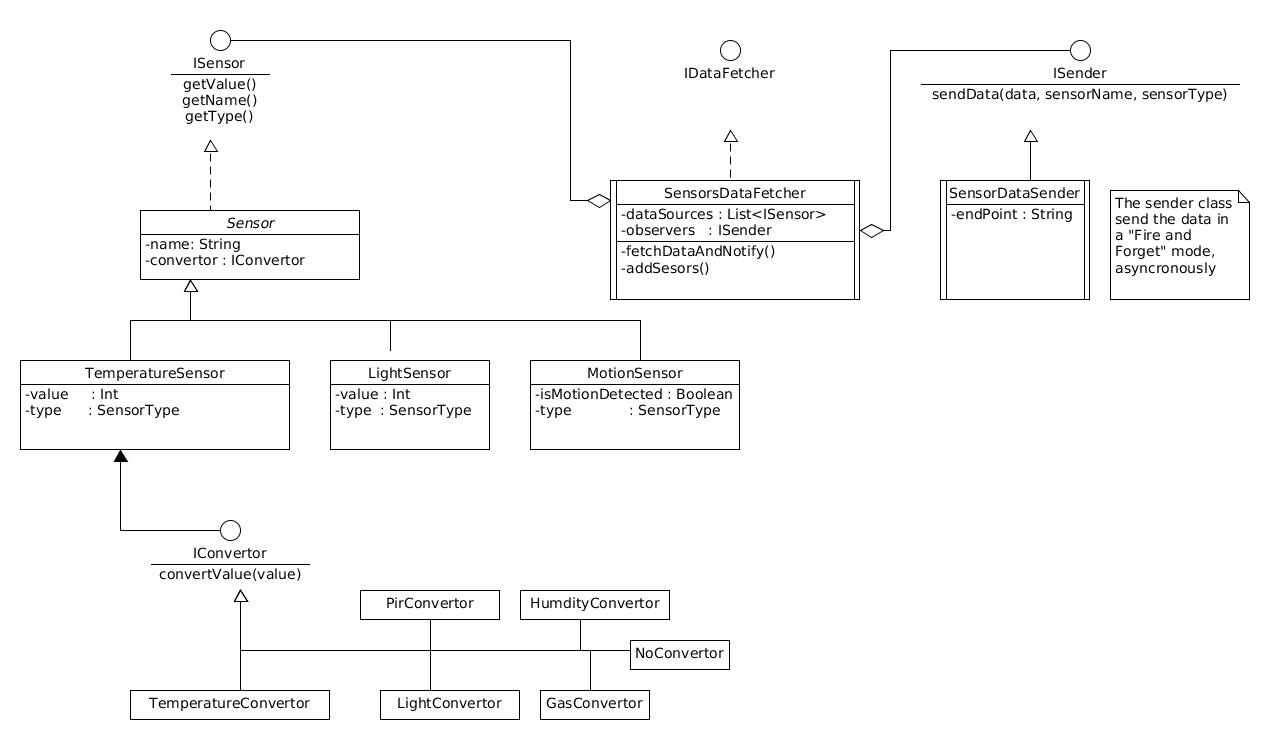
\includegraphics[width=\textwidth]{Figures/DomainModel/EmbeddedSystem/Structure.jpg}
\caption{Sistema Embedded, Struttura}
\end{figure}

Dalla struttura si possono subito individuare le entit\'a principali che sono presenti nei requisiti, in particolare la presenza di una specifica gerarchia per i sensori che condividono la stessa interfaccia che consente agilmente di ottenere il valore corrente del sensore. Sono stati inseriti solamente i sensori citati nei requisiti, ma si pu\'o facilmente intuire come qualsiasi tipo di sensore sia facilmente modellabile secondo questa struttura.

Si noti inoltre come viene anche inserita l'entit\'a IConvertor che si occoper\'a di convertire il valore di uno specifico sensore in un'unit\'a pi\'u consona per la sua gestione. Chiaramente questo viene affrontato fin da questo livello perch\'e si immagina l'operazione di conversione come un'operazione quasi istantanea e necessaria.

Infine sono presenti le entit\'a che si occupano, attivamente, di interrogare i sensori ogni intervallo di tempo predefinito e quindi inviarli altrove, In questo caso \'e stato tutto ridotto ad un singolo endpoint, anche se poi possono essere facilmente pi\'u di uno. Come si pu\'o visionare nel commento, l'invio dei dati avviene con una metodologia di tipo \textit{fire and forget}, quindi non avvengono reinvii dei dati e vengono ignorati eventuali errori. Chiaramente tutto questo \'e dovuto all'idea che i cicli di invio siano abbastanza brevi da potersi permettere eventuali perdite.

\paragraph{Interazione}

\begin{figure}[H]
\centering
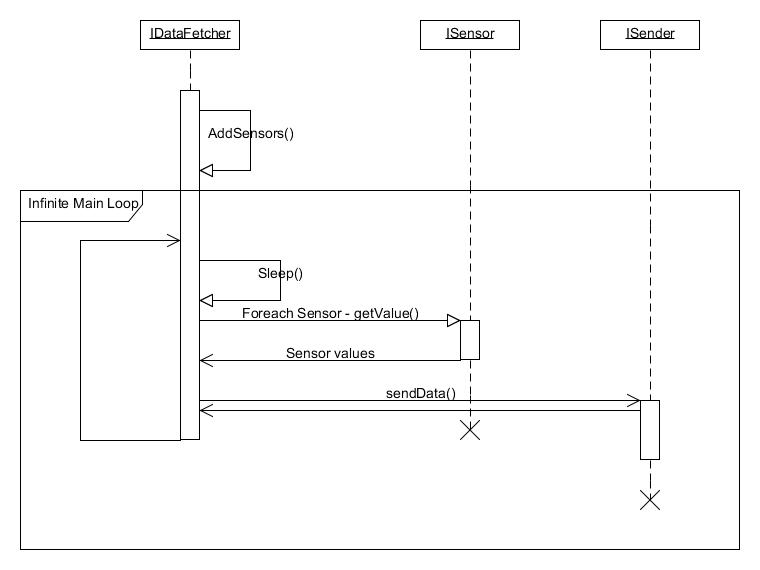
\includegraphics[width=\textwidth]{Figures/DomainModel/EmbeddedSystem/Interaction.jpg}
\caption{Sistema Embedded, Interazione}
\end{figure}

Prima di iniziare si vuole evidenziare come viene riportato solamente un diagramma di interazione perch\'e \'e presente solamente un'entit\'a attiva, ma nel futuro potrebbero esserci pi\'u task e quindi saranno necessari pi\'u diagrammi dell'interazione.

Nello schema di interazione vengono evidenziate le varie fasi del Sistema, in particolare la fase iniziale di setup dove, conoscendo quali sensori sono presenti, questi vengono aggiunti nella memoria dell'entit\'a principale in modo che poi in seguito siano facilmente interrogabili.

Terminata la fase di \textit{Init} inizia il loop infinito che appunto aspetta inizialmente un piccolo lasso di tempo e poi va a interrodage iterativamente tutti i sensori che sono stati aggiunti precedentemente, raccoglie i dati e interroga asincronamente l'entit\'a di invio, per poi ricominciare il ciclo stesso.

\paragraph{Comportamento}

\begin{figure}[H]
\centering
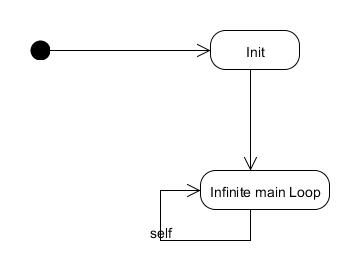
\includegraphics[scale=0.5]{Figures/DomainModel/EmbeddedSystem/Behaviour.jpg}
\caption{Sistema Embedded, Comportamento}
\end{figure}


Nel diagramma del comportamento semplicemente viene riportato quanto \'e stato precedentemente discusso semplicemente attraverso una state machine.

\subsubsection{Server}

\paragraph{}La parte server \'e quella pi\'u importante di tutto il sistema in quanto \'e quella che concentra tutta la logica applicativa del sistema stesso.

\begin{figure}[pH]
\centering
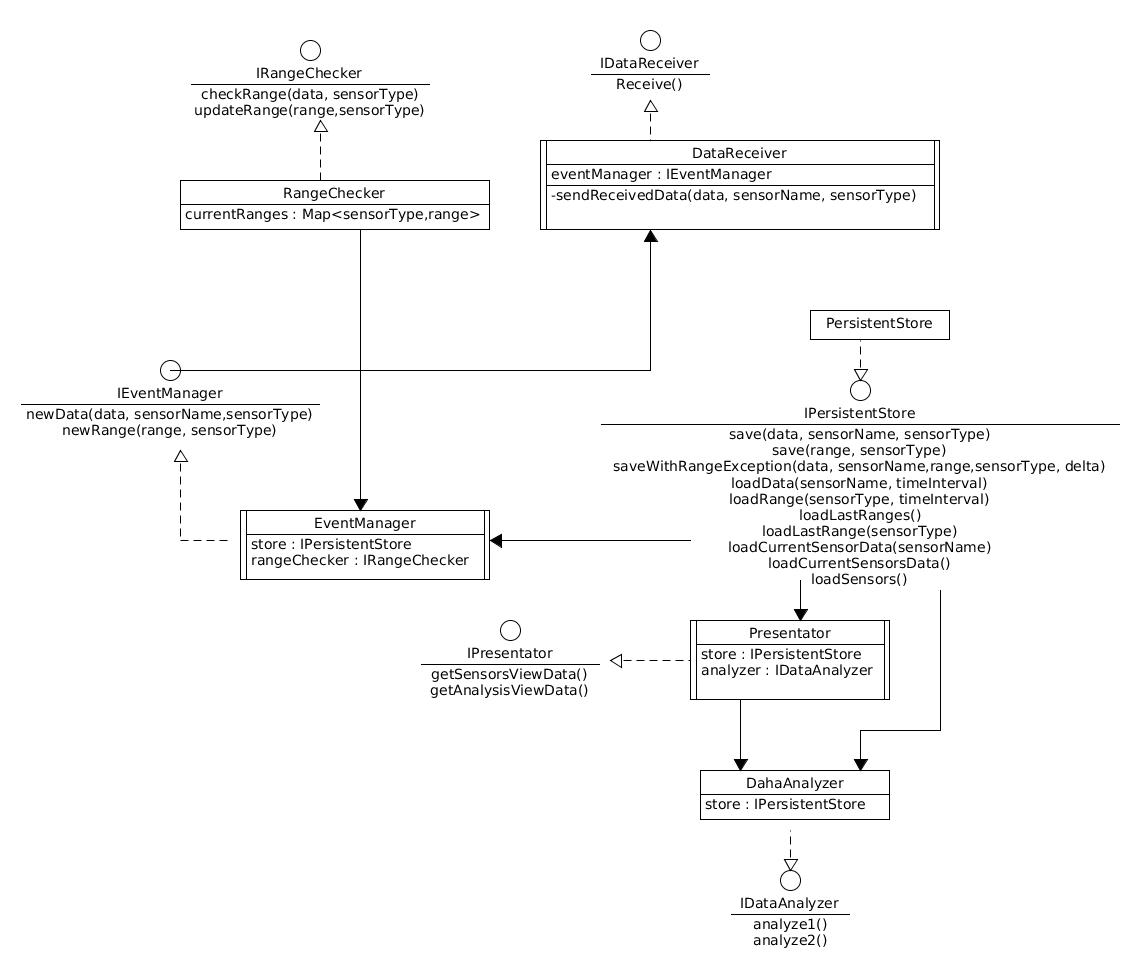
\includegraphics[width=\textwidth,height=\textheight,keepaspectratio]{Figures/DomainModel/Server/Structure.jpg}
\caption{Server, Struttura}
\end{figure}

\afterpage{\clearpage}

\newpage

\paragraph{Struttura}

Le entit\'a principali di questo schema sono:
\begin{itemize}
  \item IPersistentStore, che si occuper\'a di salvare opportunamente i dati provenienti dai sensori e dall'utente
  \item IDataReceiver, che sar\'a sempre in ascolto di ogni messaggio proveniente dal sistema embedded e quindi notificher\'a opportunamente il sistema ad ogni nuovo arrivo
  \item IPresentator che si occuper\'a di ottenere i dati necessari per le viste da mostrare all'utente quanto una nuova richiesta viene inoltrata.
\end{itemize}

Chiaramente ogniuna di queste entit\'a \'e in parte citata nei casi d'uso.

Si veda i diagrammi dell'interazione per i dettagli di come avviene la comunicazione di tutte queste entit\'a al fronte di garantire il funzionamento e il soddisfacimento dei requisiti.

\paragraph{Interazione}

\begin{figure}[H]
\centering
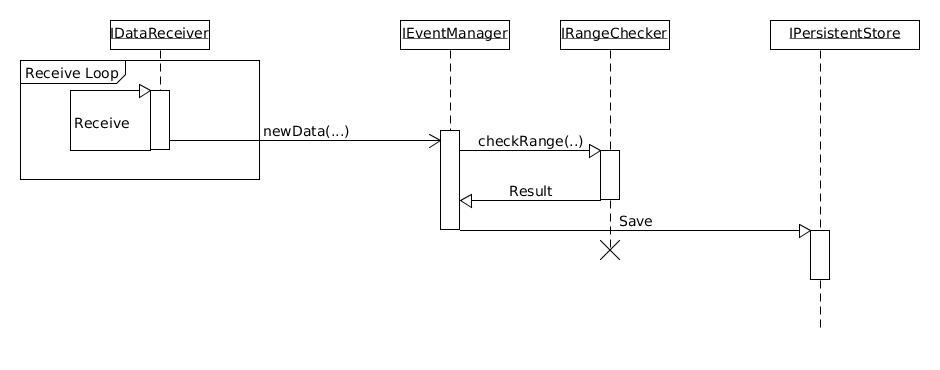
\includegraphics[width=\textwidth]{Figures/DomainModel/Server/NewDataInteraction.jpg}
\caption{Server, Interazione, Dati dai Sensori}
\end{figure}

Abbiamo deciso di omettere la parte di inizializzazione del sistema in questa fase anche perch\'e sar\'a meglio defita nell'analisi del problema dovendo aggiungere entit\'a che non sono direttamente correlate con i requisiti principali ma con requisiti non funzionali.

Nello schema sovrastante si pu\'o osservare l'interazione nel caso i sensori emettano un nuovo valore. Si vuole porre particolare enfasi su come l'entit\'a che riceve i dati rimane sempre in ascolto di nuovi arrivi delegando, tramite una chiamata asincrona alle altre entit\'a il compito di salvare i dati appena arrivati.

\noindent\rule[0.5ex]{\linewidth}{1pt}

\begin{figure}[H]
\centering
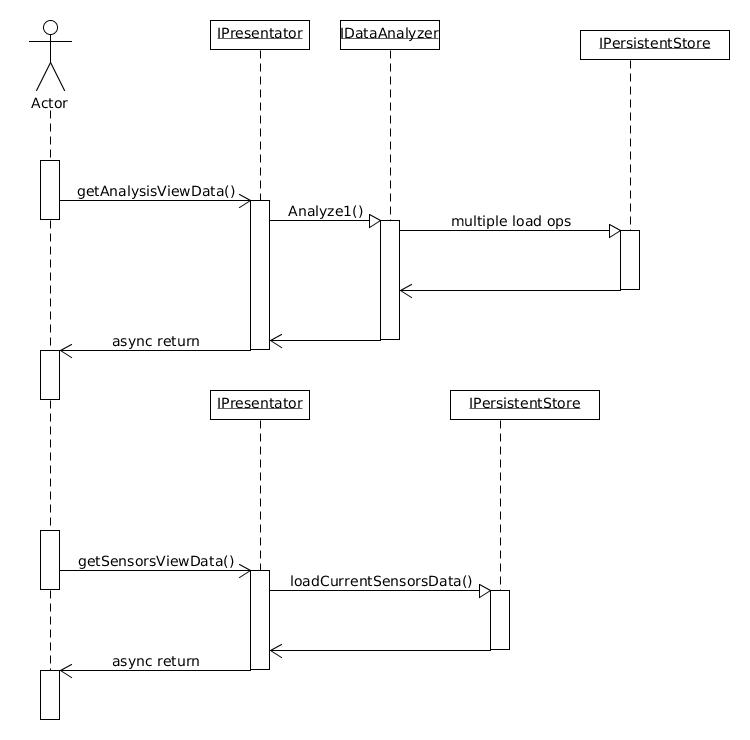
\includegraphics[width=\textwidth]{Figures/DomainModel/Server/GetOperationInteraction.jpg}
\caption{Server, Interazione, Richiesta Visualizzazione Dati}
\end{figure}

In quest'altro schema dell'interazione si pu\'o osservare che entit\'a vengono conivolte a fronte di una chiamata di visualizzazione dati da parte dell'utente. Anche in questo caso la chiamata iniziale \'e stata effettuata in maniera asincrona in modo da lasciare libero il sistema di rispondere ad eventuali altre richieste e gestirle concorrentemente.

\noindent\rule[0.5ex]{\linewidth}{1pt}

\begin{figure}[H]
\centering
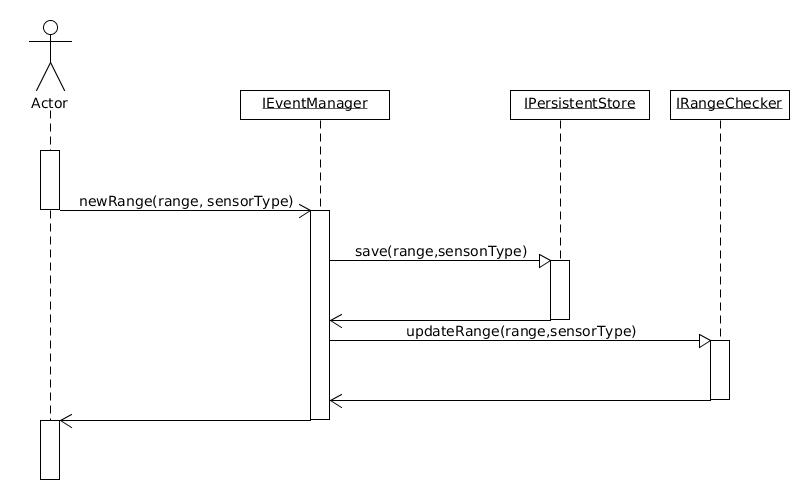
\includegraphics[width=\textwidth]{Figures/DomainModel/Server/NewRangeInteraction.jpg}
\caption{Server, Interazione, Nuovo Range}
\end{figure}

In questo caso invece viene illustata l'interazione per quanto riguarda la richiesta da parte dell'utente dell'inserimento di un nuovo range. Si vede come la chiamata questa volta arriva all'entit\'a che gestisce gli eventi essendo questo effettivamente un caso incui avviene un cambiamento nei dati e quindi tutto va gestito appropriatamente per evitare i conflitti.

\paragraph{Comportamento}

\begin{figure}[H]
\centering
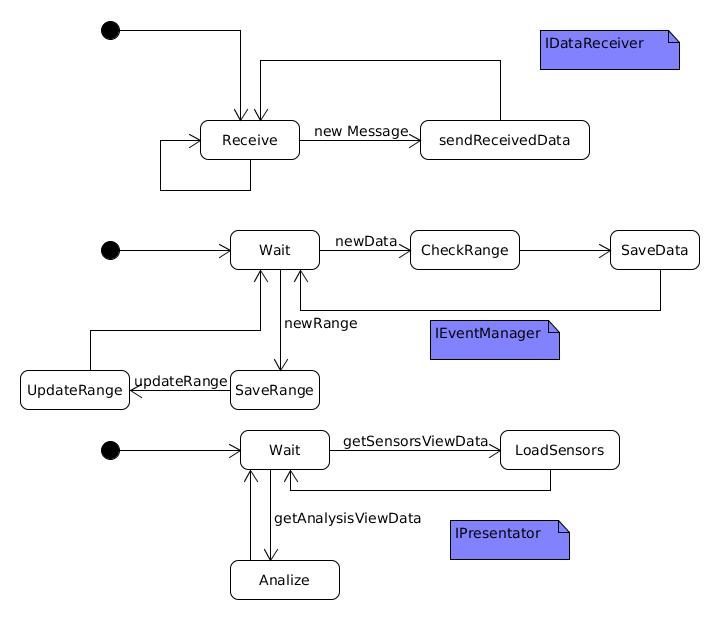
\includegraphics[width=\textwidth]{Figures/DomainModel/Server/Behaviour.jpg}
\caption{Server, Comportamento}
\end{figure}


In questa fase si mostrano le entit\'a che sono effettivamente attive e che quindi operano cambiamenti sul sistema. Si \'e deciso di omettere tutte le entit\'a che vengono solamente chiamate ed effettuano una unica operazione al fine di evitare di formalizzare troppe cose a questo livello.

Si vuole far notare inoltre come tutte queste entit\'a abbiano effettivamente uno stato di attesa di un qualche messaggio o evento. Questo aspetto pu\'o essere molto importante in seguito nelle scelte per la progettazione.

\newpage

\subsubsection{Web Site}

\paragraph{}Dopo un'attenta analisi abbiamo ritenuto superflua la necessit\'a di modellare e analizzare la parte di visualizzazione in quanto non \'e effettivamente presente nessuna business logic ma solamente la parte che effettua le richieste di dati alle parti precedenti e visualizza tutto su schermo.

La documentazione relativa a questa parte si limiter\'a solamente a come utilizzare poi il software attraverso l'interfaccia.

Possiamo per\'o pensare di definire i link a cui l'interfaccia dovr\'a rispondere appropriatamente attraverso una pagina web. Questo ci consente di impostare comunque dei test che esulano dal contenuto della pagina, ma ci garantiscono che questa sia effettivamente online in maniera automatica.

gli URL scelti sono:
\begin{itemize}
  \item \textit{http://...../DomoticRoom/Status}
  \item \textit{http://...../DomoticRoom/NewRange}
  \item \textit{http://...../DomoticRoom/Analysis}
\end{itemize}

\subsection{Piani di Test}

In questa fase saranno presenti i piani di test che vengono costruiti sulla base dei modelli precedenti, ancora privi di implementazione. Ci\'o \'e possibile perch\'e a questo punto abbiamo gi\'a individuato le interfaccie delle entiti\'a principali e le loro operazioni pubbliche.

Chiaramente a questo punto la maggior parte dei test non possono funzionare perch\'e manca l'implementazione. Anche in questa fase si divide il tutto sulle 3 parti precedenti.

\subsubsection{Sistema Embedded}
\subsubsection{Server}
\subsubsection{Web Site}
